\chapter{Feature Engineering và các model xử lý dữ liệu dạng văn bản}
 % Tên của chương
 \label{Chapter2}

\section{Các bước xử lý một bài toán học máy (MLP)}
Bất kỳ hệ thống thông minh nào về cơ bản đều bao gồm các bước bắt đầu từ việc nhập dữ liệu thô, sử dụng các kỹ thuật để sắp xếp, xử lý, thiết kế các đặc trưng (feature) và thuộc tính có ý nghĩa từ dữ liệu này. Sau đó, chúng ta thường sử dụng các kỹ thuật như mô hình thống kê hoặc các mô hình học máy để xây dựng các mô hình với mục đích giải quyết yêu cầu đặt ra. Một quy trình tiêu chuẩn điển hình dựa trên mô hình tiêu chuẩn công nghiệp CRISP-DM được mô tả như hình \ref{pic2.1}

\begin{figure}[h!]
	\centering
	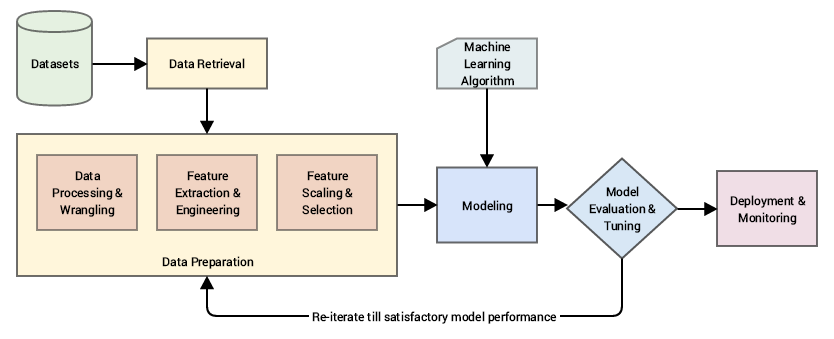
\includegraphics[width=1\textwidth]{
		mlp.png
	}
	\caption[Mô hình tiêu chuẩn công nghiệp CRISP-DM]{
		Mô hình tiêu chuẩn công nghiệp CRISP-DM \label{pic2.1}
	}
\end{figure}

\section{Giới thiệu về Feature Engineering}
Feature Engineerning là một giai đoạn không thể thiếu trong quá trình phát triển bất kỳ một hệ thống thông minh nào. Mặc dù hiện nay chúng ta có rất nhiều các phương pháp mới như học sâu, siêu mô hình hỗ trợ học máy tự động (automated machine learning), tuy nhiên với mỗi vấn đề cụ thể cần giải quyết luôn có những đặc trưng quan trọng hơn, có giá trị hơn để quyết định hiệu suất hệ thống của bạn.


\section{Cơ bản về đặc trưng của dữ liệu}

Một đặc trưng (feature) thường là một đại diện cụ thể trên dòng đầu tiên của dữ liệu thô, là một thuộc tính riêng lẻ, có thể đo lường và mô tả bởi một cột trong tập dữ liệu. Lấy ví dụ với một tập dữ liệu hai chiều, mỗi observation (quan sát) được mô tả bởi một hàng và mỗi đặc trưng được mô tả bởi một cột, sẽ có giá trị cụ thể cho mỗi đặc trưng của từng quan sát như hình \ref{pic2.2}

\begin{figure}[h!]
	\centering
	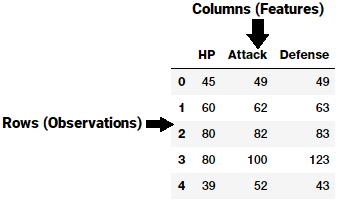
\includegraphics[width=0.5\textwidth]{
		featuresData.png
	}
	\caption[Đặc trưng của dữ liệu]{
		Đặc trưng của dữ liệu \label{pic2.2}
	}
\end{figure}

Như ví dụ ở hình trên, mỗi hàng thường biểu thị một vectơ đặc trưng và tập hợp tất cả các đặc trưng trên tất cả các quan sát tạo thành một ma trận hai chiều còn được gọi là feature-set. Thông thường, các thuật toán học máy hoạt động với các ma trận số hóa hoặc tenxo bởi vậy hầu hết các kỹ thuật feature engineering sẽ xử lý việc chuyển đổi dữ liệu thô thành các dạng biểu diễn số học giúp các thuật toán có thể dễ dàng hiểu được.

Các đặc trưng có thể chia thành hai loại chính:

\begin{itemize}
	\item \textbf{Đặc trưng thô (Raw features)}: là các đặc trưng vốn có được lấy trực tiếp từ tập dữ liệu mà không cần sử dụng thêm thao tác kỹ thuật nào
	\item \textbf{Đặc trưng phát sinh (Derived features)}: là các đặc trưng được thu được sau quá trình feature engineering, là kết quả của quá trình trích xuất và xử lý các đặc trưng có sẵn. 
\end{itemize}

\section{Kĩ thuật tạo đặc trưng dữ liệu}

Về kĩ thuật tạo đặc trưng cho dữ liệu có 3 phương pháp chính:
\begin{itemize}
	\item \textbf{Trích lọc feature}: Không phải toàn bộ thông tin được cung cấp từ một biến dự báo hoàn toàn mang lại giá trị trong việc phân loại. Do đó chúng ta cần phải trích lọc những thông tin chính từ biến đó. Chẳng hạn như trong các mô hình chuỗi thời gian chúng ta thường sử dụng kĩ thuật phân rã thời gian để trích lọc ra các đặc trưng như Ngày thành Năm, Tháng, Quí,…. Các đặc trưng mới sẽ giúp phát hiện các đặc tính chu kì và mùa vụ, những đặc tính mà thường xuất hiện trong các chuỗi thời gian
	\item \textbf{Biến đổi feature}:  Biến đổi dữ liệu gốc thành những dữ liệu phù hợp với mô hình nghiên cứu. Những biến này thường có tương quan cao hơn đối với biến mục tiêu và do đó giúp cải thiện độ chính xác của mô hình
	\item \textbf{Lựa chọn feature} : Phương pháp này được áp dụng trong những trường hợp có rất nhiều dữ liệu mà chúng ta cần lựa chọn ra dữ liệu có ảnh hưởng lớn nhất đến sức mạnh phân loại của mô hình. Các phương pháp có thể áp dụng đó là ranking các biến theo mức độ quan trọng bằng các mô hình như Random Forest, Linear Regression, Neural Network,…; Sử dụng chỉ số IV trong scorecard; Sử dụng các chỉ số khác như AIC hoặc Pearson Correlation, phương sai.
\end{itemize}

\section{Xử lý dữ liệu dạng văn bản}

\begin{enumerate}
	\item Import các thư viện cần thiết và khởi tạo một đoạn văn bản mẫu cần xử lý \lstinputlisting[style=codePython]{"Code/dependencies.py"}
	Kết quả: 
	\lstinputlisting[style=plaintext]{"Code/dependencies.txt"}
	\item
	\item Tiền xử lý văn bản \cite{WEBSITE:10}
	\begin{itemize}
		\item \textbf{Xóa thẻ tags}: Văn bản chúng ta gặp thường chứa nội dung không cần thiết như các thẻ \textbf{HTML}, không có giá trị khi phân tích. Thư viện \textbf{BeautifulSoup} là một công cụ tuyệt vời và cần thiết để xử lý trong trường hợp này.
		\item \textbf{Xóa các ký tự có dấu}:Trong bất kỳ văn bản nào, đặc biệt nếu bạn đang xử lý ngôn ngữ tiếng Anh, thường các bạn cần phải xử lý các ký tự có dấu. Do đó, chúng ta vần đảm bảo rằng các ký tự này cần được chuyển đổi và chuẩn hóa thành các ký tự ASCII
		\item \textbf{Biến đổi các từ viết tắt}: Trong tiếng Anh, các từ viết tắt về cơ bản là phiên bản rút gọn của các từ hoặc âm tiết. Những từ viết tắt của các từ hoặc cụm từ thường được tạo ra bằng cách loại bỏ các chữ cái và âm tiết. Ví dụ như: \textbf{do not -> don't, I would -> I'd}. Chuyển đổi từ dạng viết tắt thành dạng đầy đủ cũng là một bước cần thiết để chuẩn hóa văn bản.
		\item \textbf{Xóa các ký tự đặc biệt}: Các ký tự đặc biệt thường là các ký tự không phải là chữ và số, thường gây "nhiễu" cho dữ liệu của chúng ta. Thông thường, regular expressions \textbf{(regexes)} có thể được sử dụng để xử lý vấn đề này.
		\item \textbf{Từ gốc và ngữ pháp}:  Trong các ngữ cảnh khác nhau, các từ gốc thường được gắn thêm các tiền tố và hậu tố vào để đúng với ngữ pháp. Ví dụ các từ: \textbf{WATCHES, WATCHING}, and \textbf{WATCHED}. Chúng ta có thể thấy rằng chúng đều có chung từ gốc là \textbf{WATCH}.
		\item \textbf{Xóa các stopwords}: stopwords là các từ có ít hoặc không có ý nghĩa gì đặc biệt khi xây dựng các đặc trưng
	\end{itemize}
	\lstinputlisting[style=codePython]{"Code/simpleDataProcessing.py"}
	
	Kết quả:
	
	\lstinputlisting[style=plaintext]{"Code/simpleDataProcessing.txt"}

\end{enumerate}

\section{Các model phổ biến trong việc xử lý dữ liệu dạng văn bản}

\subsection{Bag of Words Model - Túi từ}
Mô hình Bag of words biểu diễn cho mỗi mẫu dữ liệu văn bản dưới dạng một vecto số trong đó mỗi chiều là một từ cụ thể trong kho dữ liệu và giá trị có thể là tần số của nó xuất hiện trong đoạn văn bản (giá trị có thể là 0 hoặc 1) hoặc thậm chí là các giá trị có trọng số. \cite{WEBSITE:10}

Tên mô hình này là Bag of words thể hiện theo đúng nghĩa đen của nó nghĩa là một túi các từ, không quan tâm đến trật tự, trình tự, ngữ pháp. \cite{WEBSITE:10}

Ví dụ về model \textbf{Bag of Words}

\lstinputlisting[style=codePython]{"Code/bagOfWords.py"}

Kết quả
\lstinputlisting[style=plaintext]{"Code/bagOfWords.txt"}

\subsection{Bag of N-Grams}
Là phân bố xác suất trên các tập văn bản\\

Cho biết xác suất của 1 câu (hoặc 1 cụm từ) thuộc 1 ngôn ngữ là bao nhiêu
Mô hình ngôn ngữ tốt sẽ đánh giá đúng các câu đúng ngữ pháp, trôi chảy hơn các cụm từ có thứ tự ngẫu nhiên \cite{NGRAM1}

Các mô hình N-grams phổ biến \cite{NGRAM}:
\begin{itemize}
	\item \textbf{Unigram}: mô hình với n=1, tức là ta sẽ tính tần suất xuất hiện của một kí tự (từ), như: “k”, “a”,…
	\item \textbf{Bigrams}: với n=2 , là mô hình được sử dụng nhiều trong việc phân tích các hình thái cho ngôn ngữ
	\item \textbf{Trigrams}:với n-3, với n càng lớn thì độ chính xác càng cao tuy nhiên đi kèm với đó thì độ phức tạp cũng lớn hơn
\end{itemize}

Mô hình N-gram \cite{NGRAM}:
Mục tiêu: Tính xác suất của 1 câu hoặc 1 cụm từ:
\begin{itemize}
	\item Để tính xác suất của một câu: W1W2...Wk...Wn, Theo công thứ Bayes \cite{NGRAM} \ref{2.1}:
	\begin{equation}
		p(w_1...w_n) = \frac{count(w_1...w_n)}{N} \label{2.1} 
	\end{equation}
	
	\item Tuy nhiên, công thức trên có độ phức tạp lớn, vì vậy người ta thường sử dụng công thức Markov \cite{NGRAM} \ref{2.2}:
	\begin{equation}
		p(w_1...w_n) = p(w_1) * p(w_2|w_1) * p(w_3|w_1w_2)  *...*p(w_n|w_1...w_(n-1)) \label{2.2} 
	\end{equation}
\end{itemize}

Ví dụ về model \textbf{Bag of N-grams}:

\lstinputlisting[style=codePython]{"Code/nGram.py"}

Kết quả \ref{pic2.3}: 
\begin{figure}[h!]
	\centering
	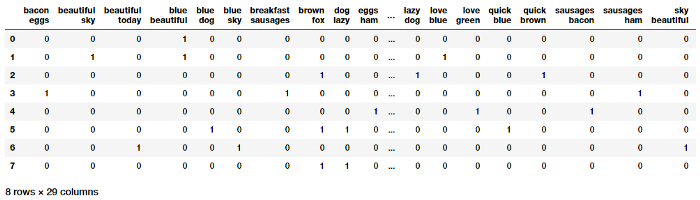
\includegraphics[width=1\textwidth]{
			ngramFigures.png
		}
	\caption[Kết quả của model Bag of N-grams]{
			Kết quả của model Bag of N-grams  \cite{WEBSITE:11} \label{pic2.3}
		}
\end{figure}

\subsection{TF-IDF - Term Frequency-Inverse Document Frequency}
TF-IDF là viết tắt của Term Frequency-Inverse Document Frequency.\\
Hiểu một cách đơn giản nó là sự kết hợp của tần số xuất hiện của một từ trong một mẫu và nghịch đảo của tần số của từ đó trong toàn bộ tập dữ liệu\\
Kỹ thuật này được phát triển để đánh giá kết quả cho các truy vấn trong công cụ tìm kiếm và hiện tại nó là một phần không thể thiếu trong xử lý ngôn ngữ tự nhiên \cite{WEBSITE:11}\\
Về mặt toán học có thể định nghĩa như sau \cite{WEBSITE:10} \ref{2.3}:

\begin{equation}
	tfidf(w,D) = tf(w,D)*idf(w,D)=tf(w,D)*log(\frac{C}{df(w)}) \label{2.3}
\end{equation}

Theo công thức trên, \textbf{tfidf(w,D)} là một 'score'. TF-IDF cho từ \textbf{w} trong mẫu \textbf{D}. Thuật ngữ \textbf{tf(w,D)} đại diện cho tần số của từ \textbf{w} xuất hiện trong mẫu \textbf{D} có thể lấy được từ mô hình \textbf{Bag of words}. Thuật ngữ \textbf{idf(w,D)} là tần số nghịch đảo của \textbf{w} có thể tính là \textbf{log} của tổng số mẫu dữ liệu xuất hiện từ \textbf{w}. \\
Mô hình này có thể có rất nhiều biến thể khác nhau, tuy nhiên chúng đều cho kết quả khá giống nhau. 

Ví dụ về model \textbf{TF-IDF}: 

\lstinputlisting[style=codePython]{"Code/tfidf.py"}

Kết quả \ref{pic2.4}:

\begin{figure}[h!]
	\centering
	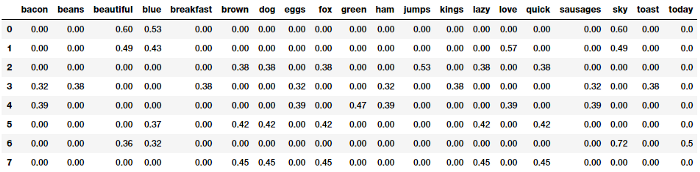
\includegraphics[width=1\textwidth]{
		tfidfFigures.png
	}
	\caption[Kết quả của model TF-IDF]{
		Kết quả của model TF-IDF   \cite{WEBSITE:11} \label{pic2.4}
	}
\end{figure}

\subsection{Document Similarity}
Document Similarity (hay độ tương tự của văn bản) là quá trình sử dụng số liệu dựa trên khoảng cách hoặc độ tương tự có thể sử dụng để xác định mức độ tương đương của một văn bản với bất kỳ văn bản nào khác dựa trên các đặc trưng được trích xuất ra từ \textbf{bag of words} hoặc \textbf{tf-idf}.\\
Sự tương tự giữa các mẫu dữ liệu trong một kho văn bản cũng được hiểu là sự tương tự giữa từng cặp mẫu trong toàn bộ kho văn bản đó

Có rất nhiều công thức có thể sử dụng để tính toán độ tương tự này như khoảng cách cosin, khoảng cách euclide, khoảng cách manhattan...  \cite{WEBSITE:11}

Ví dụ sử dụng \textbf{cosine} để tính toán độ tương tự 
\lstinputlisting[style=codePython]{"Code/cosine.py"}

Kết quả \ref{pic2.5}:
\begin{figure}[h!]
	\centering
	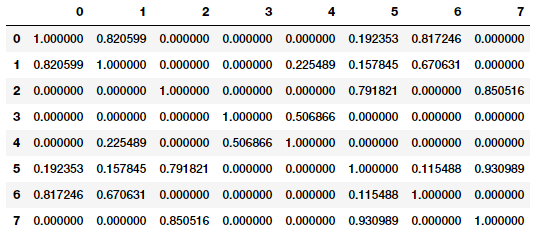
\includegraphics[width=1\textwidth]{
		cosine.png
	}
	\caption[Kết quả của model  Document Similarity.]{
		Kết quả của model  Document Similarity.   \cite{WEBSITE:11} \label{pic2.5}
	}
\end{figure}

Về cơ bản, khoảng cách cosin cung cấp cho chúng ta một số liệu biểu thị góc giữa 2 vecto đặc trưng tương ứng của từng mẫu. Góc giữa hai mẫu càng gần nhau thì độ tương tự của hai mẫu đó càng lớn như được mô tả trong hình dưới đây\\

\begin{figure}[h!]
	\centering
	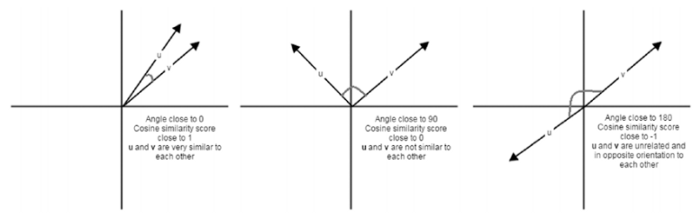
\includegraphics[width=1\textwidth]{
		cosin1.png
	}
	\caption[Độ tương tự của hai mẫu theo khoảng cách cosine]{
		Độ tương tự của hai mẫu theo khoảng cách cosine.   \cite{WEBSITE:11} \label{pic2.5}
	}
\end{figure}
%
%\section{Trích lọc đặc trưng cho dữ liệu dạng văn bản}
%
%Dữ liệu văn bản có thể đến từ nhiều nguồn và nhiều định dạng khác nhau (kí tự thường, kí tự hoa, kí tự đặc biệt,…). Có nhiều phương pháp xử lý dữ liệu phù hợp với từng đề tài cụ thể. Ở đây chúng tôi sẽ sử dụng kĩ thuật mã hóa (tokenization)\cite{WEBSITE:3}
%
%Mã hóa đơn giản là việc chúng ta chia đoạn văn thành các câu văn, các câu văn thành các từ. 
%
%Trong mã hóa thì từ là đơn vị cơ sở. Chúng ta cần một bộ tokenizer có kích thước bằng toàn bộ các từ xuất hiện trong văn bản hoặc bằng toàn bộ các từ có trong từ điển. 
%
%Một câu văn sẽ được biểu diễn bằng một sparse vector mà mỗi một phần tử đại diện cho một từ, giá trị của nó bằng 0 hoặc 1 tương ứng với từ không xuất hiện hoặc có xuất hiện.
%
%Chúng ta sử dụng các túi từ (bags of words) để tạo ra một vector có độ dài bằng độ dài của tokenizer và mỗi phần tử của túi từ sẽ đếm số lần xuất hiện của một từ trong câu và sắp xếp chúng theo một vị trí phù hợp trong vector. Bên dưới là code minh họa cho quá trình này.
%
%\lstinputlisting[style=codePython]{"Code/tokenization.py"}
%
%Quá trình này có thể được mô tả như hình \ref{pic2.3}:
%\begin{figure}[h!]
%	\centering
%	\includegraphics[width=1\textwidth]{
%		tokenization.png
%	}
%	\caption[Biểu diễn kĩ thuật mã hóa]{
%		Biểu diễn kĩ thuật mã  \label{pic2.3}
%	}
%\end{figure}
%
%Cách biểu diễn theo túi từ có hạn chế đó là chúng ta không phân biệt được 2 câu văn có cùng các từ bởi túi từ không phân biệt thứ tự trước sau của các từ trong một câu. Chặng như ‘you have no dog’ và ‘no, you have dog’ là 2 câu văn có biểu diễn giống nhau mặc dù có ý nghĩa trái ngược nhau. Chính vì thế phương pháp N-gram sẽ được sử dụng thay thế.
%
%\lstinputlisting[style=codePython]{"Code/nGram.py"}
%
%
%Những từ hiếm khi được tìm thấy trong tập văn bản (corpus) nhưng có mặt trong một văn bản cụ thể có thể quan trọng hơn. Do đó cần tăng trọng số của các nhóm từ ngữ để tách chúng ra khỏi các từ phổ biến. Cách tiếp cận này được gọi là TF-IDF (Term Frequency - Inverse Document Frequency)
%
%Các chỉ số chính đánh giá tần xuất xuất hiện của một từ trong toàn bộ tập văn bản là idf và tfidf được tính theo công thức \ref{tdf} \ref{tfidf}:
%
%\begin{equation}
%	idf(t,D) = log(\frac{|D|}{df(d,t) + 1})\\ \label{tdf}
%\end{equation}
%
%\begin{equation}
%	tfidf(t,d,D) = tf(d,d) x idf(i, D) \label{tfidf}
%\end{equation}
%
%Ở đây:
%\begin{itemize}
%	\item \textbf{|D|}: là số lượng các văn bản trong tập văn bản
%	\item \textbf{df(d,t)}: là số lượng các văn bản là từ t xuất hiện
%	\item \textbf{tf(dt)}: là tần suất các từ xuất hiện trong một văn bản
%\end{itemize}
%Như vậy một từ càng phổ biến khi idf càng nhỏ và tfidf càng lớn.
%Do đó để tính \textbf{tfidf} cho các từ trong văn bản, ta có thể làm như sau:
%
%\lstinputlisting[style=codePython]{"Code/tfidf.py"}
%
%Kết quả:
%
%\lstinputlisting[style=plaintext]{"Code/tfidf.txt"}
%
%Ta có thể thấy từ "I" xuất hiện ở toàn bộ các câu và không mang nhiều ý nghĩa của chủ đề của câu nên có thể coi là một stopword. Bằng phương pháp lọc cận trên của tần suất xuất hiện từ trong văn bản là 90\% ta đã loại bỏ được từ này khỏi dictionary.